\subsection{Desempeño global}
\label{sec:desempeno-global}

\eegnet{} alcanza una exactitud de $0.634$ en el protocolo intra-sujeto y de $0.761$ en \loso{}
(tabla~\ref{tab:baseline-global} y figura~\ref{fig:resultados-baseline}).

\begin{table}[H]
\centering
\caption{Desempeño de \eegnet{} bajo los dos protocolos de validación.
Media sobre 54 sujetos de la media de tres semillas por sujeto; el símbolo
$\pm$ es la desviación típica entre los 54 sujetos.}
\label{tab:baseline-global}
\begin{tabular}{lccc}
\toprule
\textbf{Protocolo} & \textbf{Exactitud} & \textbf{Kappa} & \textbf{Particiones} \\
\midrule
Intra-sujeto (por sesión) & $0.634 \pm 0.107$ &  & $54 \times 3$ semillas \\
\loso{}                   & $0.761 \pm 0.119$ & $0.521 \pm 0.237$ & $54 \times 3$ semillas \\
\bottomrule
\end{tabular}
\end{table}

La exactitud \loso{} es coherente con la única referencia inter-sujeto sobre este conjunto,
$74.15$\,\% con validación dejando un sujeto fuera \cite{kwon2020}, que difiere en modelo,
preprocesamiento y conjunto de prueba y se toma como contexto y no como referencia directa. La
réplica de la línea base CSP+LDA de los autores obtuvo 0.714 y 0.730 frente a los 0.701 y 0.722
publicados \cite{lee2019} (sección~\ref{sec:replica}). No se detecta sesgo de clase: la
exactitud agregada de los $54$ \textit{folds} es 0.778 en una clase y 0.743 en la otra, diferencia
no significativa por sujeto (Wilcoxon pareado, $p = 0.49$).

\begin{figure}[H]
\centering
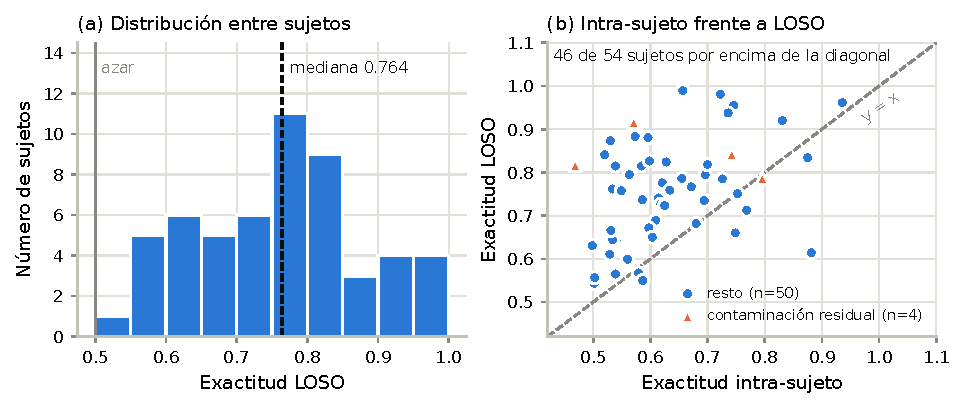
\includegraphics[width=\textwidth]{resultados_baseline.pdf}
\caption{Desempeño de \eegnet{} sobre los 54 sujetos (media de tres semillas). (a) Distribución de la
exactitud \loso{}; la línea continua marca el azar y la discontinua la mediana. (b) Exactitud
intra-sujeto frente a \loso{}; los puntos por encima de la diagonal son sujetos mejor decodificados
con un modelo entrenado en \emph{otras} personas. En naranja, los cuatro sujetos con contaminación
residual. La exactitud intra-sujeto depende del procedimiento de selección del modelo
(subsección~\ref{sec:seleccion-intra}).}
\label{fig:resultados-baseline}
\end{figure}

